\chapter{THIẾT KẾ CƠ SỞ DỮ LIỆU}
\label{ch:05}

\section{Sơ đồ thực thể liên kết (ERD) tổng quan 11 bảng chuẩn 3NF}
Cơ sở dữ liệu được thiết kế theo mô hình quan hệ RDBMS đạt chuẩn 3NF, loại bỏ tối đa dị thường dữ liệu (Hình~\ref{fig:erd}).

\begin{figure}[htbp]
    \centering
    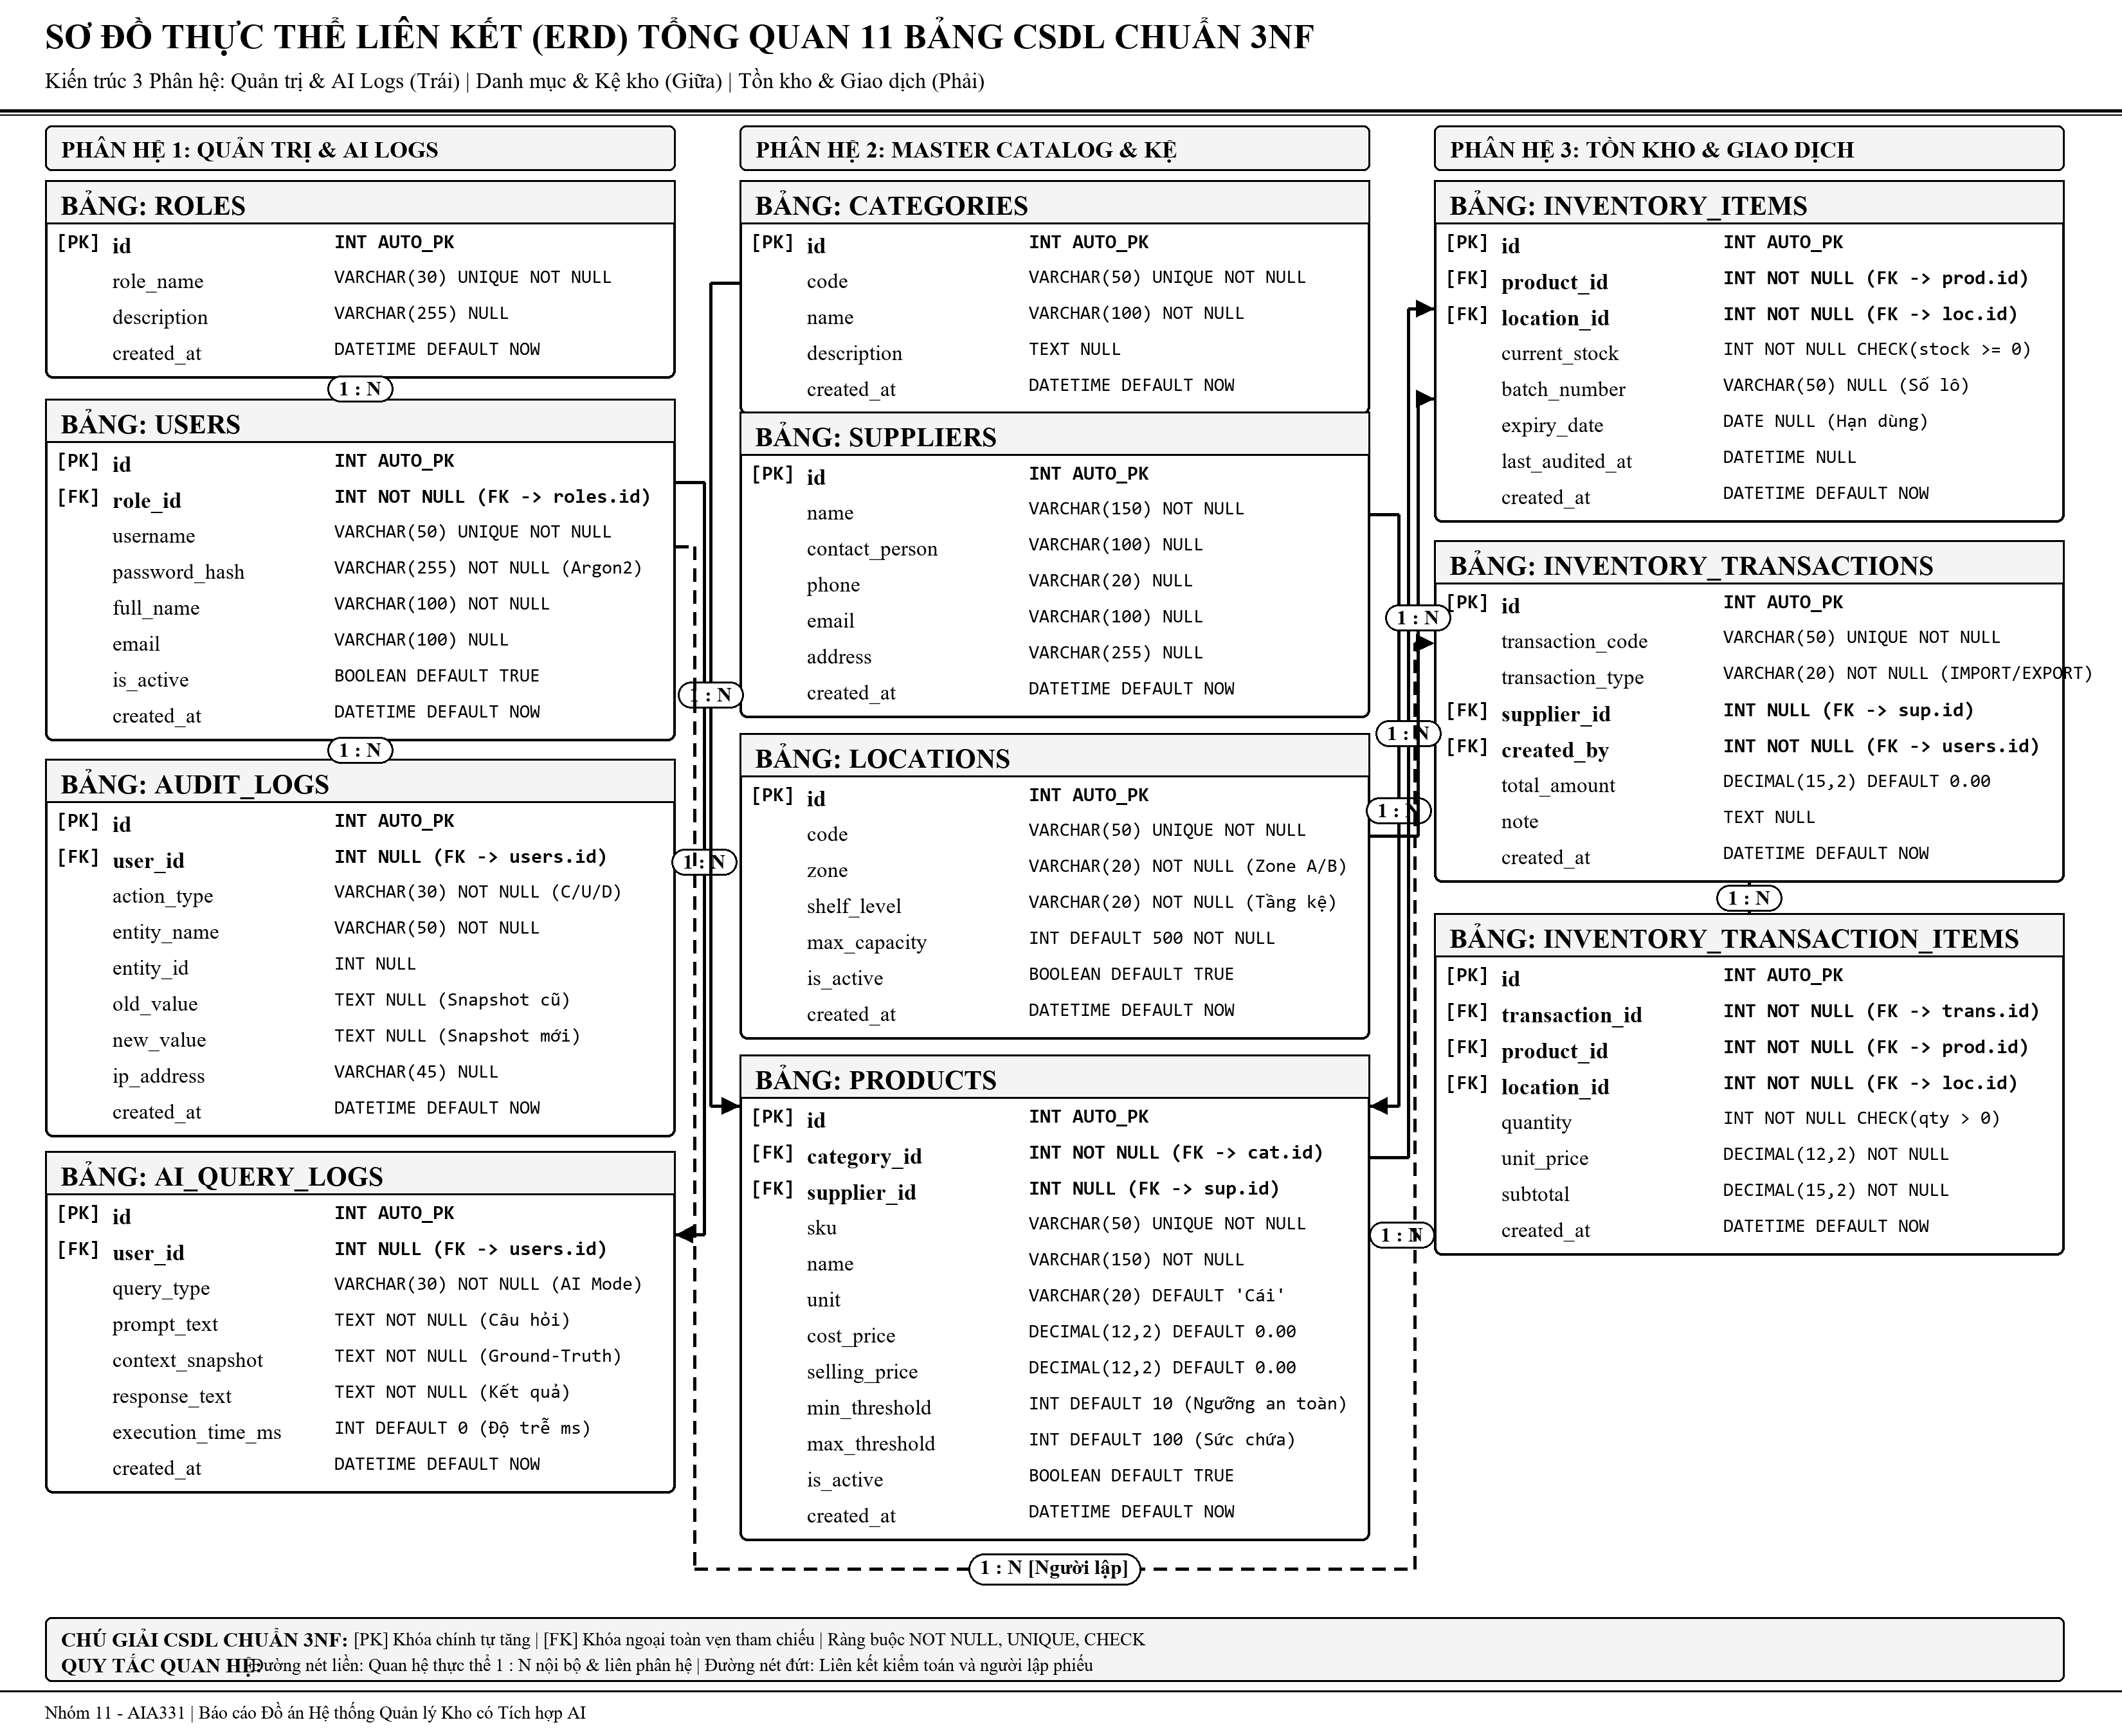
\includegraphics[width=0.98\textwidth]{03_so_do_erd_11_bang.png}
    \caption{Sơ đồ thực thể liên kết (ERD) tổng quan 11 bảng CSDL chuẩn 3NF (Nhóm 11)}
    \label{fig:erd}
\end{figure}

\section{Thiết kế chi tiết các phân hệ cơ sở dữ liệu}
Cấu trúc 11 bảng CSDL được phân rã chi tiết thành 3 phân hệ nghiệp vụ độc lập:

\subsection{Phân hệ Quản trị người dùng, Phân quyền RBAC và AI Logs}
Quản lý vai trò phân quyền, tài khoản mật khẩu băm Argon2, vết kiểm toán Audit Trail và nhật ký prompt AI (Hình~\ref{fig:erd_users_ai}).
\begin{figure}[htbp]
    \centering
    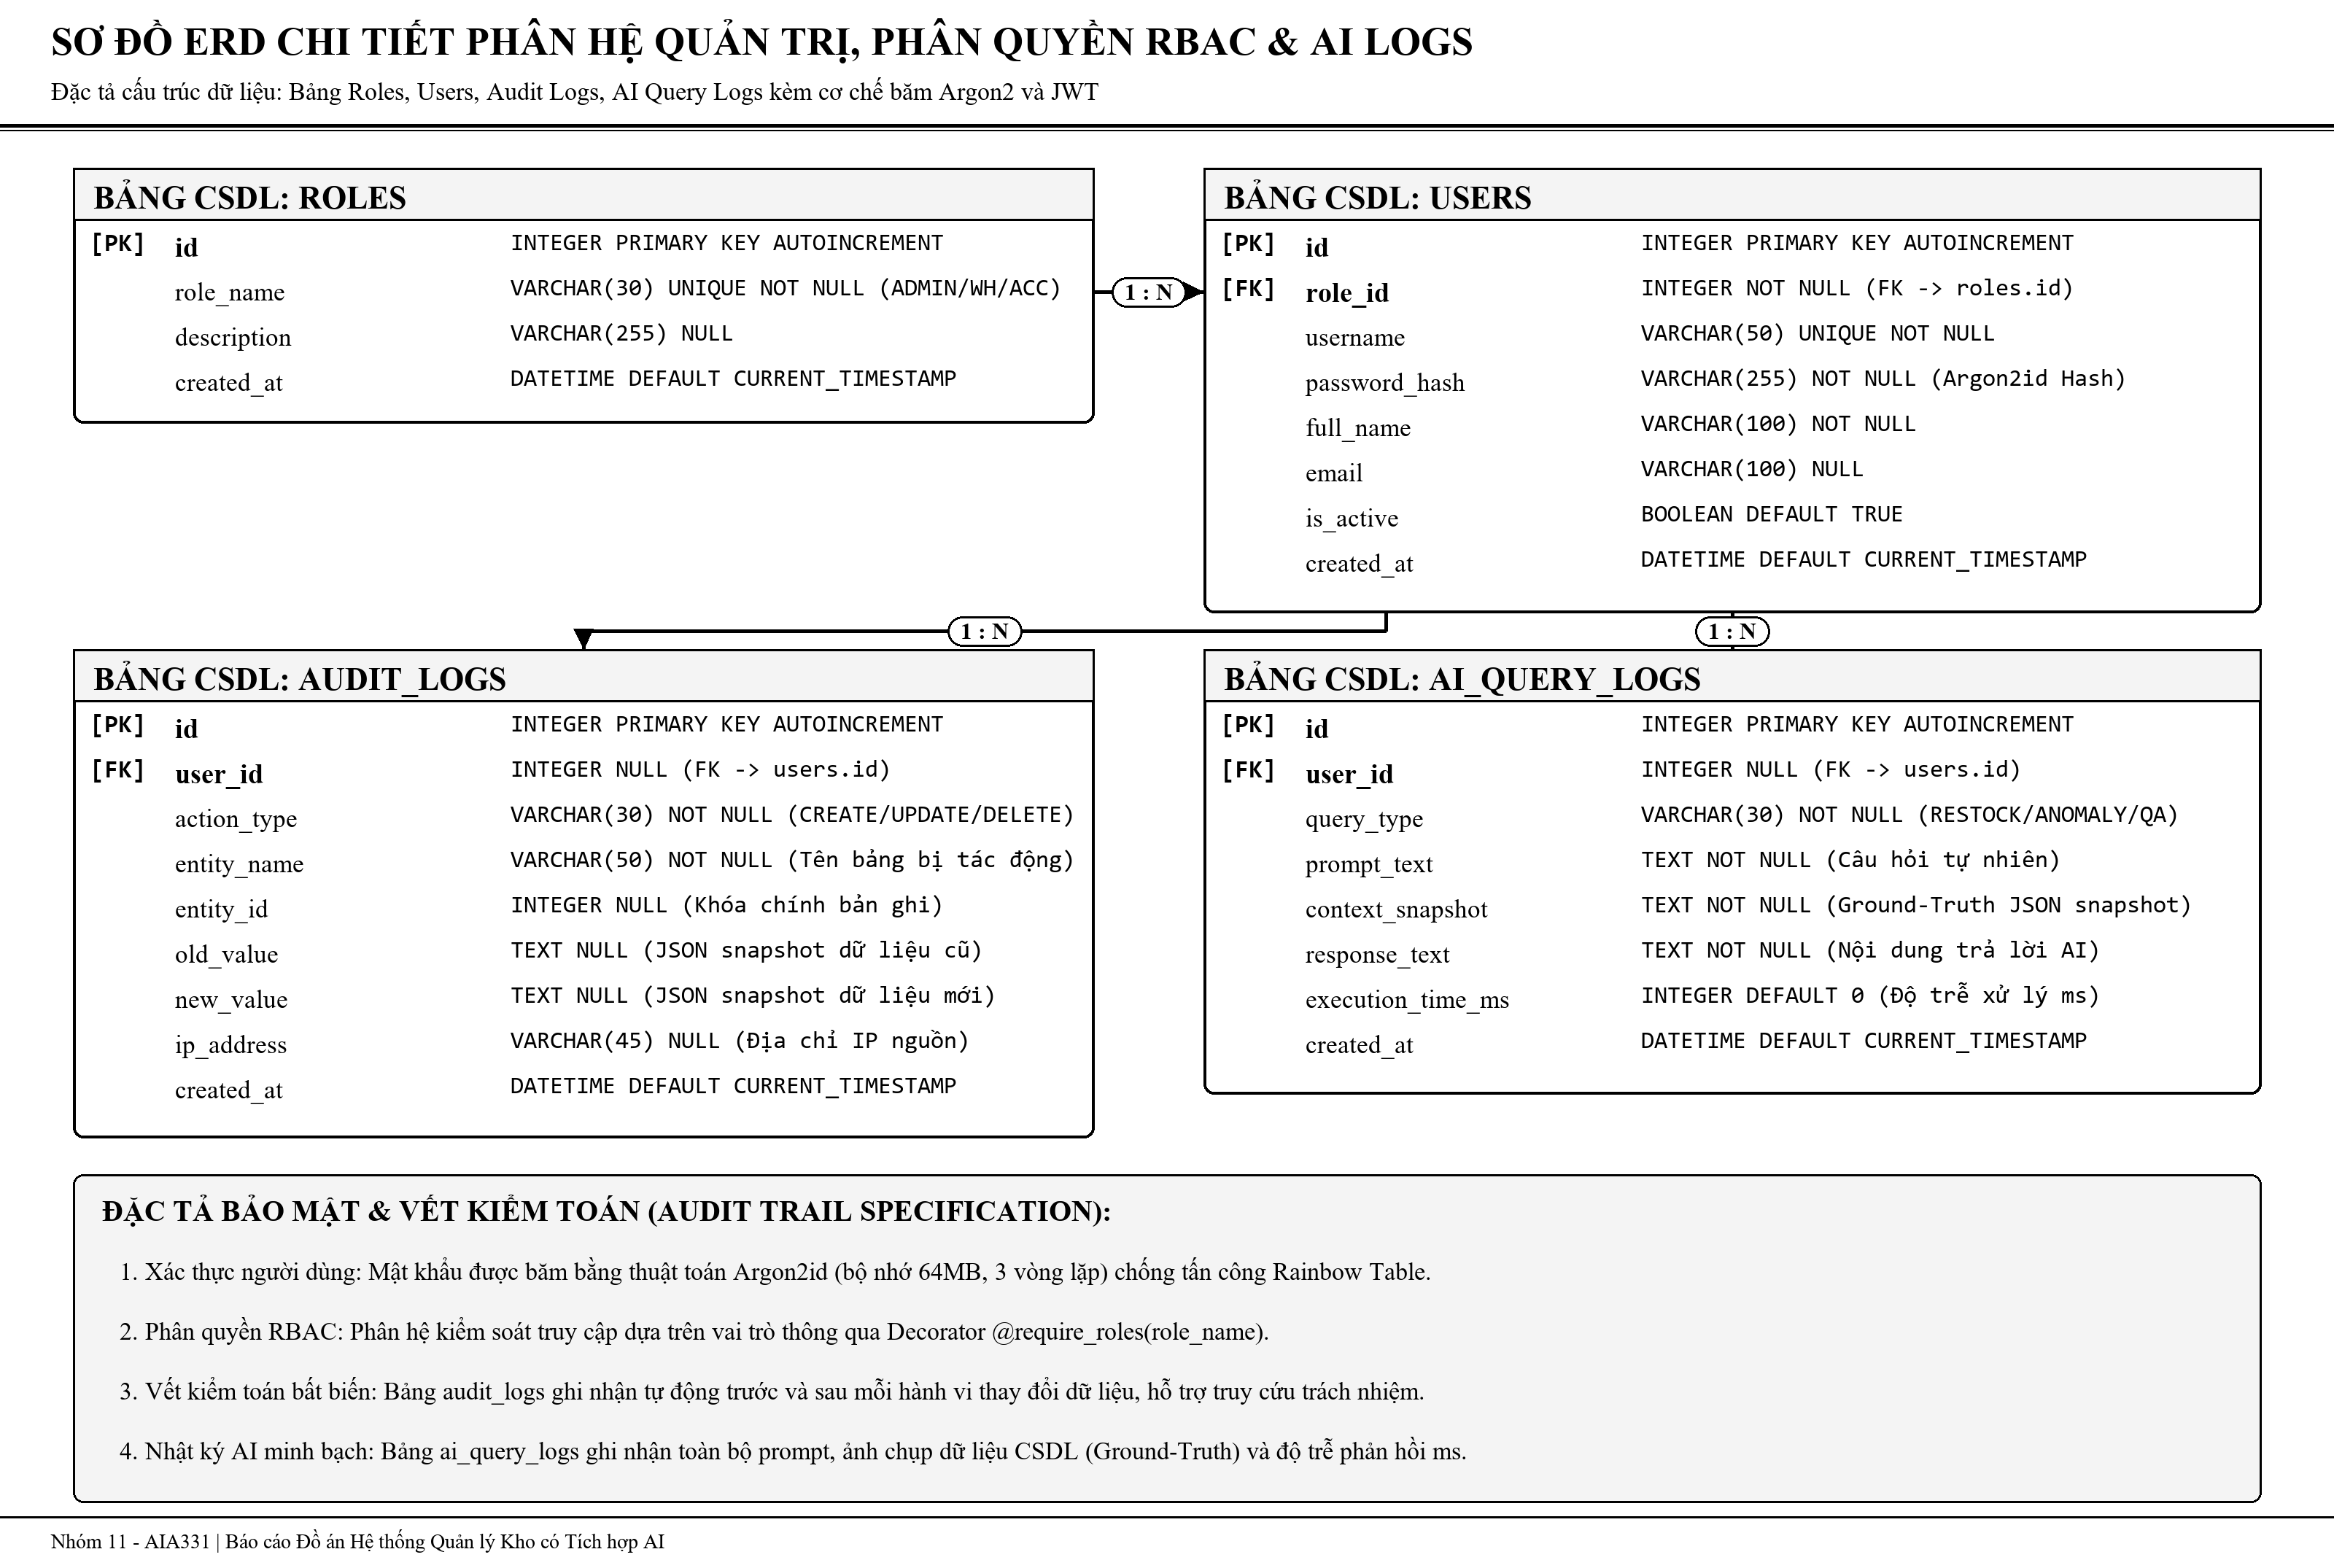
\includegraphics[width=0.95\textwidth]{03a_erd_nhom_nguoi_dung_ai.png}
    \caption{Sơ đồ ERD chi tiết phân hệ Quản trị người dùng, Phân quyền RBAC và AI Logs (Nhóm 11)}
    \label{fig:erd_users_ai}
\end{figure}

\subsection{Phân hệ Danh mục Hàng hóa, Nhà cung cấp và Vị trí Kệ kho}
Quản lý danh mục hàng hóa, nhà cung cấp, mã vị trí vật lý theo cấu trúc Zone-Shelf-Level và mã SKU duy nhất (Hình~\ref{fig:erd_master}).
\begin{figure}[htbp]
    \centering
    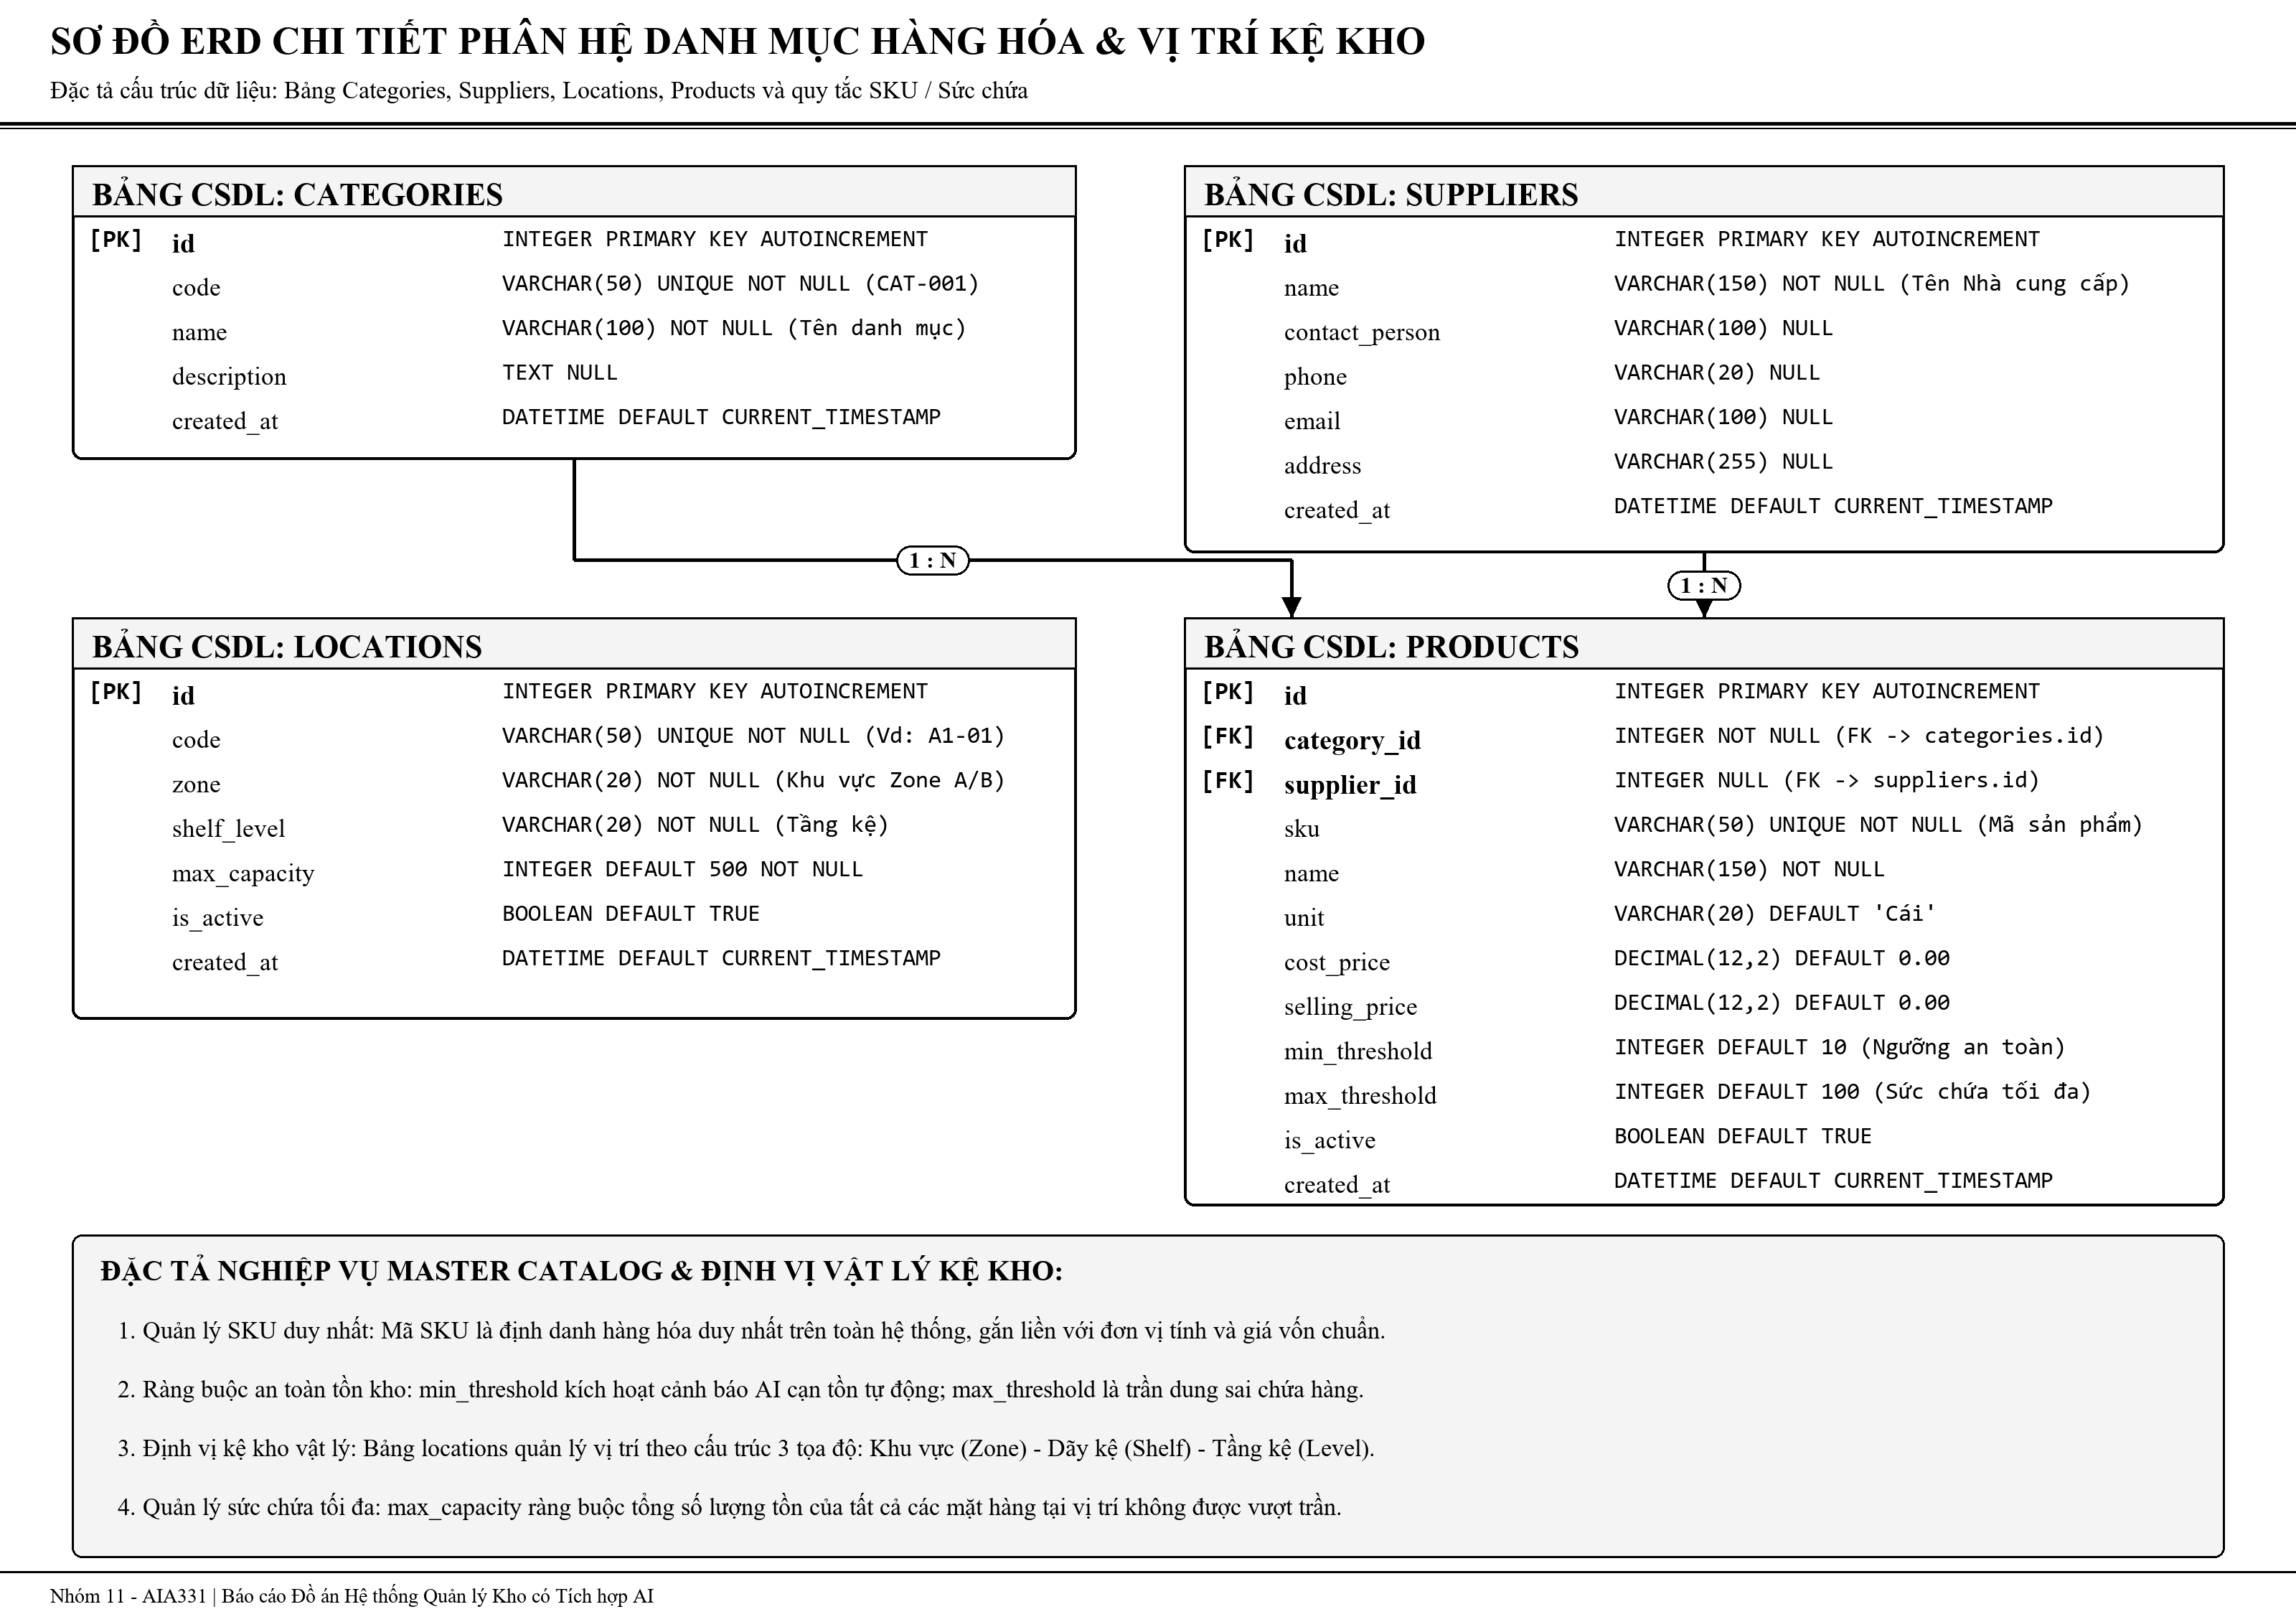
\includegraphics[width=0.95\textwidth]{03b_erd_nhom_danh_muc_kho.png}
    \caption{Sơ đồ ERD chi tiết phân hệ Danh mục Hàng hóa, Nhà cung cấp và Vị trí Kệ kho (Nhóm 11)}
    \label{fig:erd_master}
\end{figure}

\subsection{Phân hệ Quản lý Tồn kho Khả dụng và Giao dịch Xuất Nhập kho}
Quản lý số lượng tồn thực tế, số lô sản xuất, hạn sử dụng và chi tiết phiếu giao dịch có khóa dòng an toàn (Hình~\ref{fig:erd_trans}).
\begin{figure}[htbp]
    \centering
    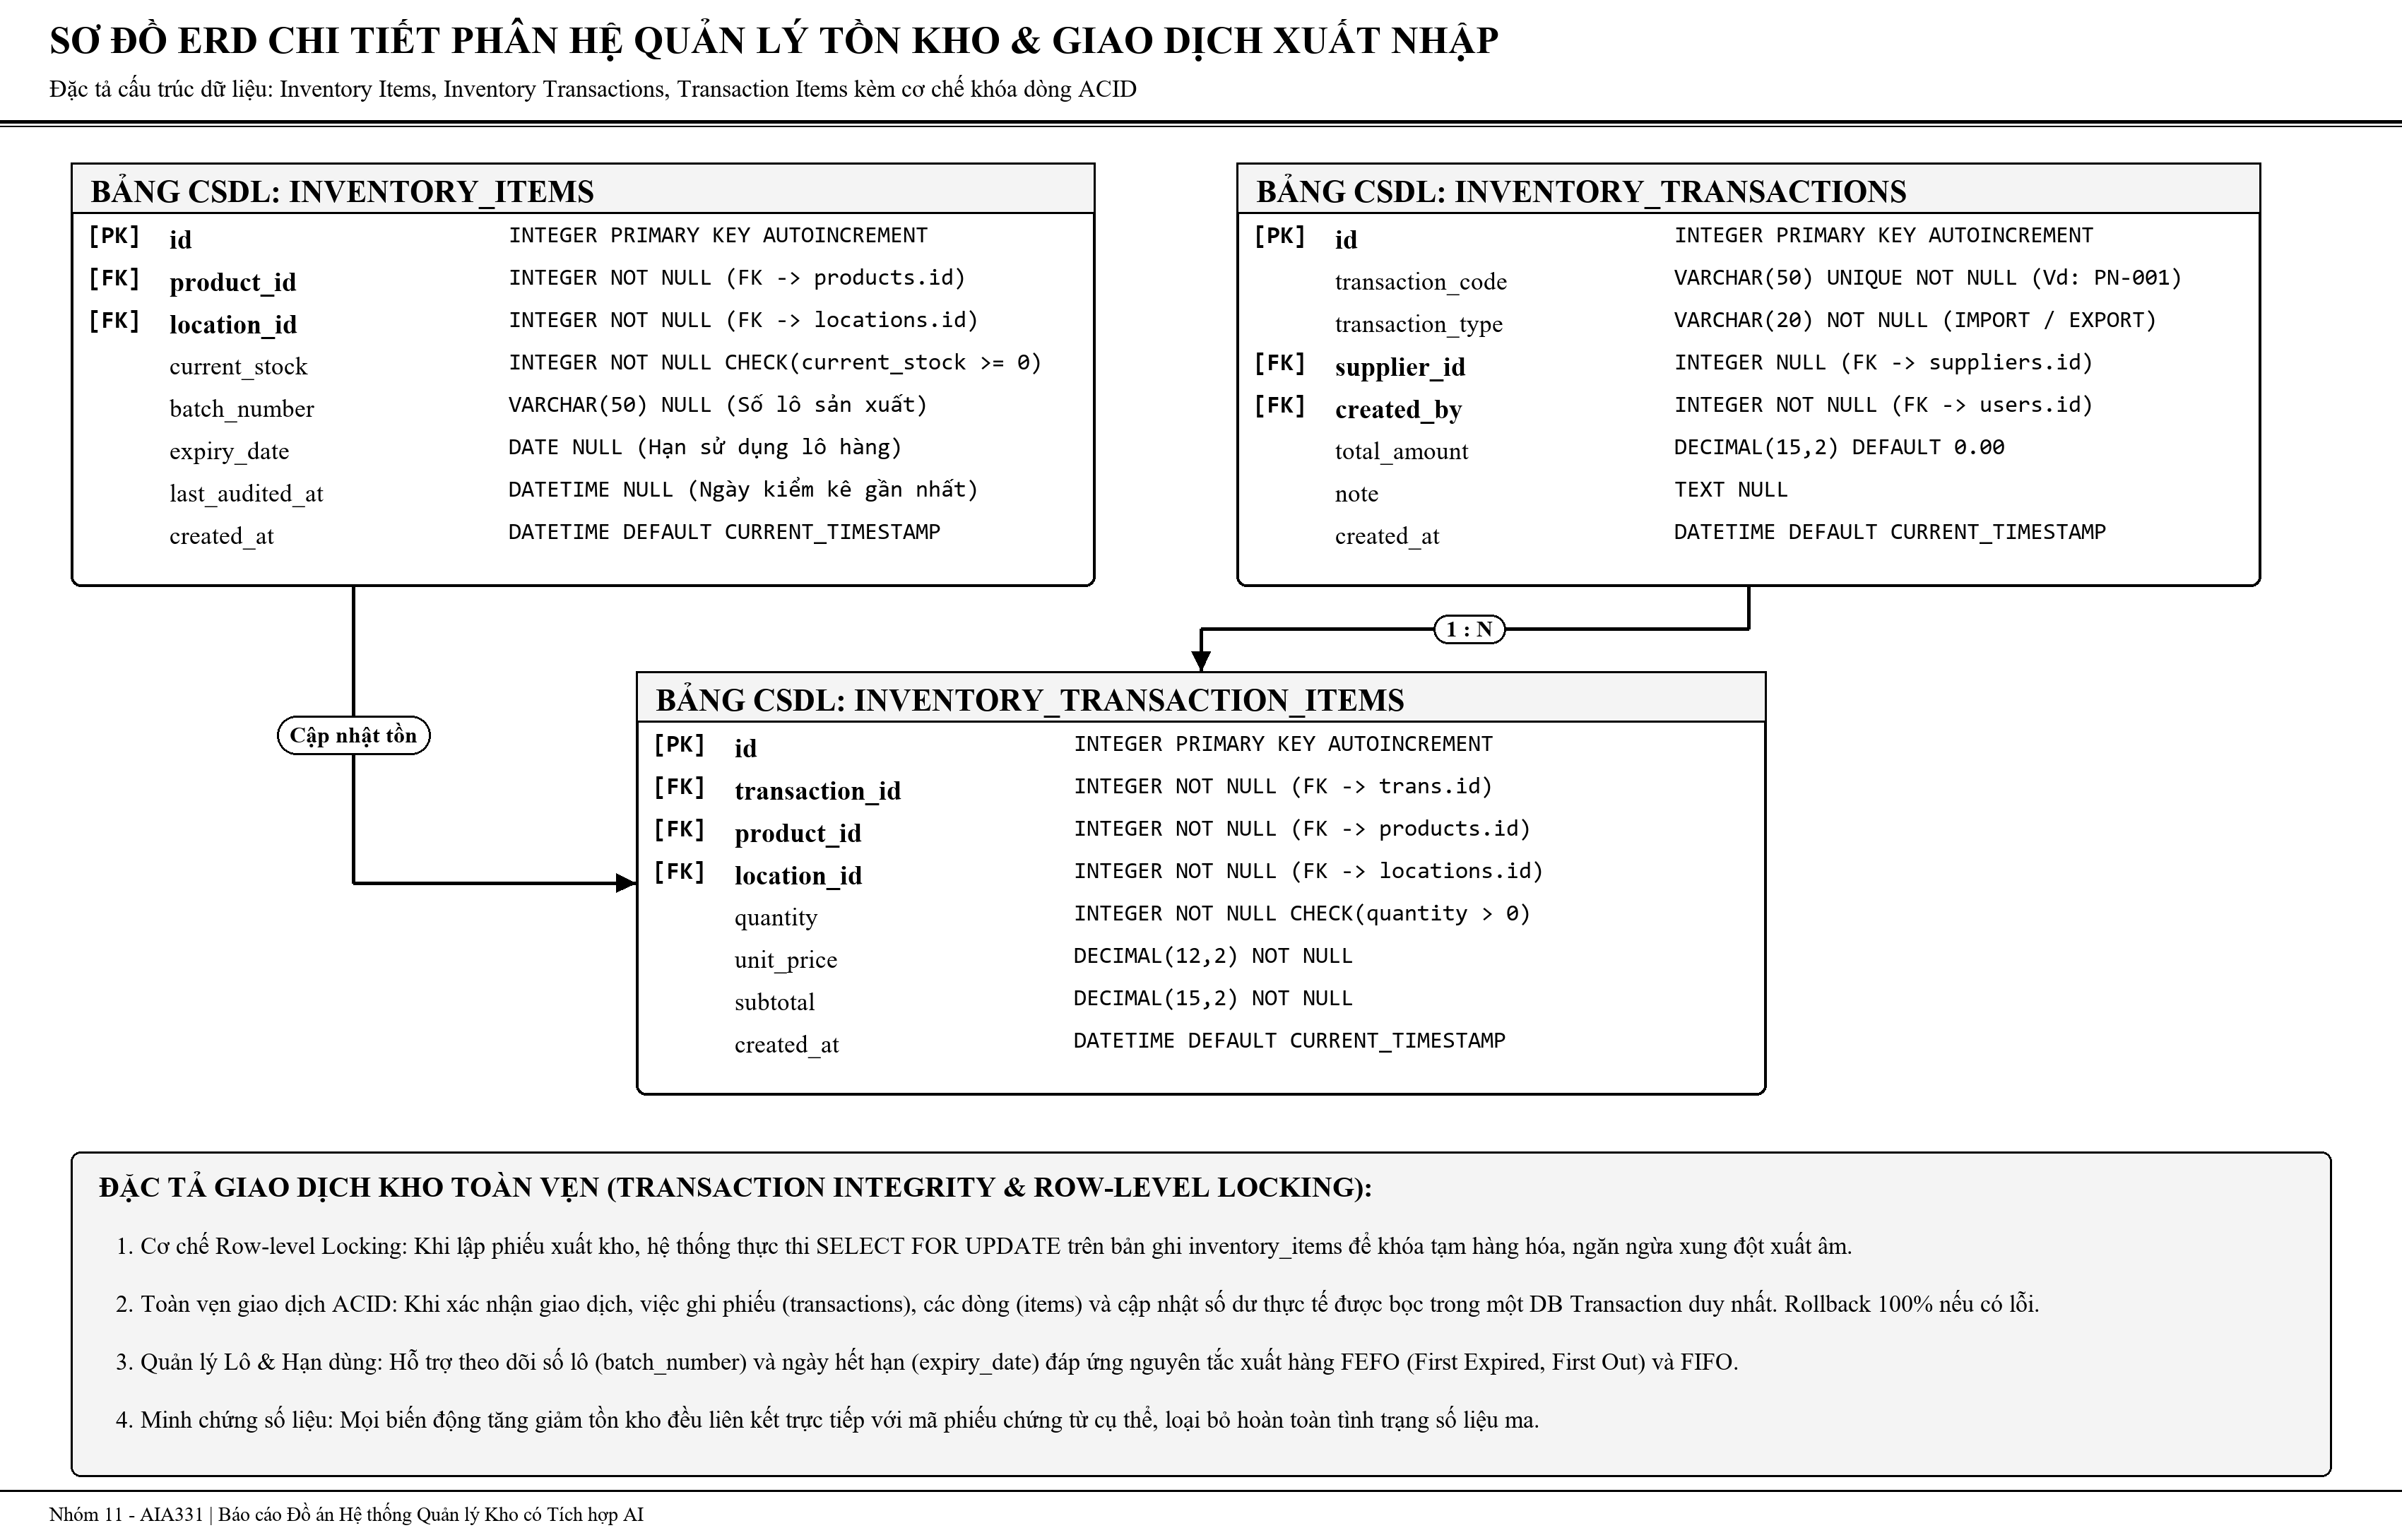
\includegraphics[width=0.95\textwidth]{03c_erd_nhom_ton_kho_giao_dich.png}
    \caption{Sơ đồ ERD chi tiết phân hệ Quản lý Tồn kho Khả dụng và Giao dịch Xuất Nhập kho (Nhóm 11)}
    \label{fig:erd_trans}
\end{figure}

\section{Danh mục 11 bảng cơ sở dữ liệu quan hệ}
Bao gồm: \texttt{roles}, \texttt{users}, \texttt{categories}, \texttt{suppliers}, \texttt{locations}, \texttt{products}, \texttt{inventory\_items}, \texttt{inventory\_transactions}, \texttt{inventory\_transaction\_items}, \texttt{audit\_logs}, \texttt{ai\_query\_logs}.
